\documentclass[10pt,a4paper]{article}
\usepackage[utf8]{inputenc}
\usepackage[T1]{fontenc}
\usepackage{lmodern}
\usepackage[margin=1in]{geometry}
\usepackage{parskip}
\usepackage{caption}
\usepackage{amsmath, amsfonts,amssymb, enumerate}
\usepackage{graphicx}
\usepackage{hyperref}
\hypersetup{
    colorlinks=true,
    linkcolor=black,
    filecolor=magenta,      
    urlcolor=black,
    pdftitle={Overleaf Example},
    pdfpagemode=FullScreen,
    }
\usepackage{float}
\usepackage[shortlabels]{enumitem }
\usepackage[frenchb]{babel}
\graphicspath{ {../img/} }

\begin{document}
\tableofcontents
\vspace{30mm}
\section{Exploration des données}
A partir de statistiques descriptives simples, expliquez votre approche initiale pour aborder ce jeu de données. Illustrez votre réponse avec quelques graphiques et/ou cartes.

\vspace{5mm}
$\textbf{Réponse : }$

Nous disposons de trois caractéristiques dans le jeu de données : un identifiant utilisateur ($\sf{user\_id}$),
des données temporelles ($\sf{timestamp\_client}$) et des données spatiales ($\sf{lat, lon}$). Ces données forment des séries-temporelles de localisation.
L'objectif de ce projet est de déterminer le lieu d'habitation d'un utilisateur. Nous aborderons
ce jeu de données en analysant l'aspect spatial et temporel des données.

\vspace{5mm}
\subsection{Description générale}

Nous vérifions d'abord la présence de doublons et valeurs manquantes dans le jeu de données.

Le jeu de données peut être résumé comme :


\begin{table}[H]
    \begin{center}
        \begin{tabular}{|c|c|}
            \hline
            Statistique             & Valeur                        \\
            \hline
            Taille de l'échantillon & 19985                         \\
            Nombre d'utilisateurs   & 12                            \\
            Période de tracking     & 698 jours et 15 h 10 min 21 s \\
            \hline
        \end{tabular}
        \caption{\label{tab:table1}Statistiques Générales}
    \end{center}
\end{table}

\begin{figure}[H]
    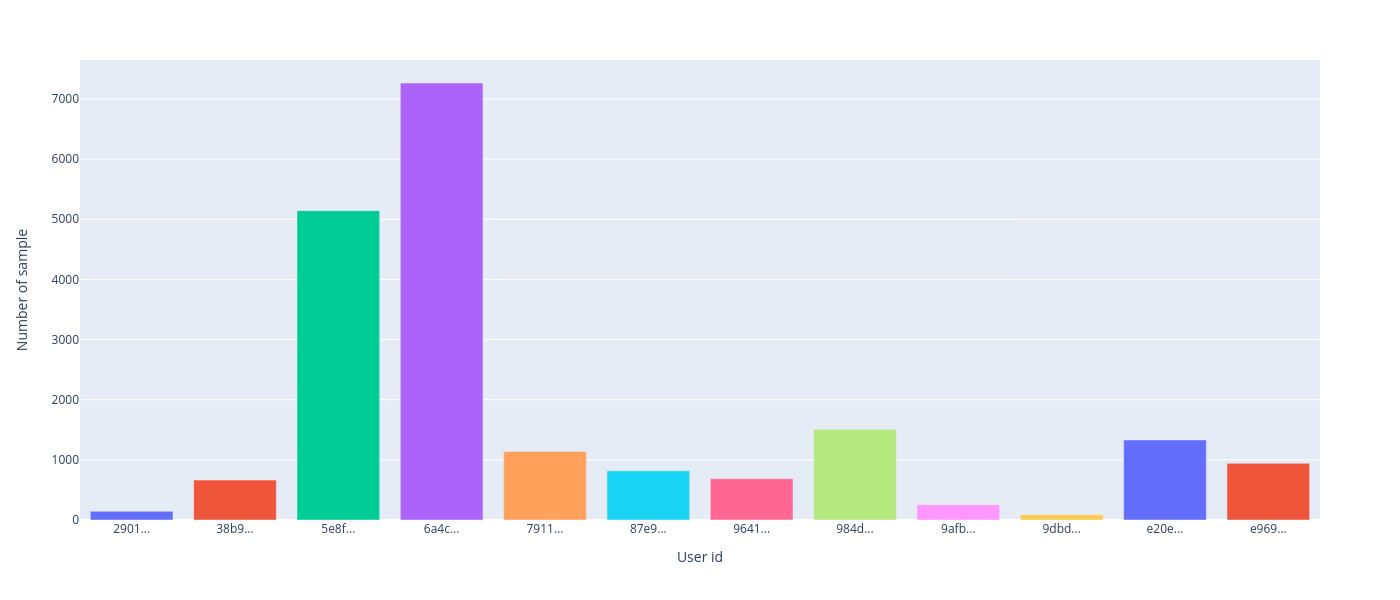
\includegraphics[scale=0.3]{sample_per_user}
    \centering
    \caption{Distribution des mesures par utilisateur}
    \label{fig:figure1}
\end{figure}

\begin{table}[H]
    \begin{center}
        \begin{tabular}{|c|c|}
            \hline
            Statistique & Valeur \\
            \hline
            Moyenne     & 1665.4 \\
            Mediane     & 879.5  \\
            Ecart-type  & 2212.9 \\
            \hline
        \end{tabular}
        \caption{\label{tab:table2}Statistiques de la distribution des mesures par utilisateur}
    \end{center}
\end{table}

D'aprés la Figure 1 on remarque que les données ne sont pas réparties équitablement entre les utilisateurs.
Il y a une forte dispersion des valeurs autour de la moyenne (${\sigma=2219.9}$). Pour certains utilisateurs
il peut être difficile de prédire le lieu d'habitation de manière précise.

\vspace{5mm}
\subsection{Description temporelle}

Dans cette partie nous explorons la caractéristique temporelle du jeu de données.

\begin{figure}[H]
    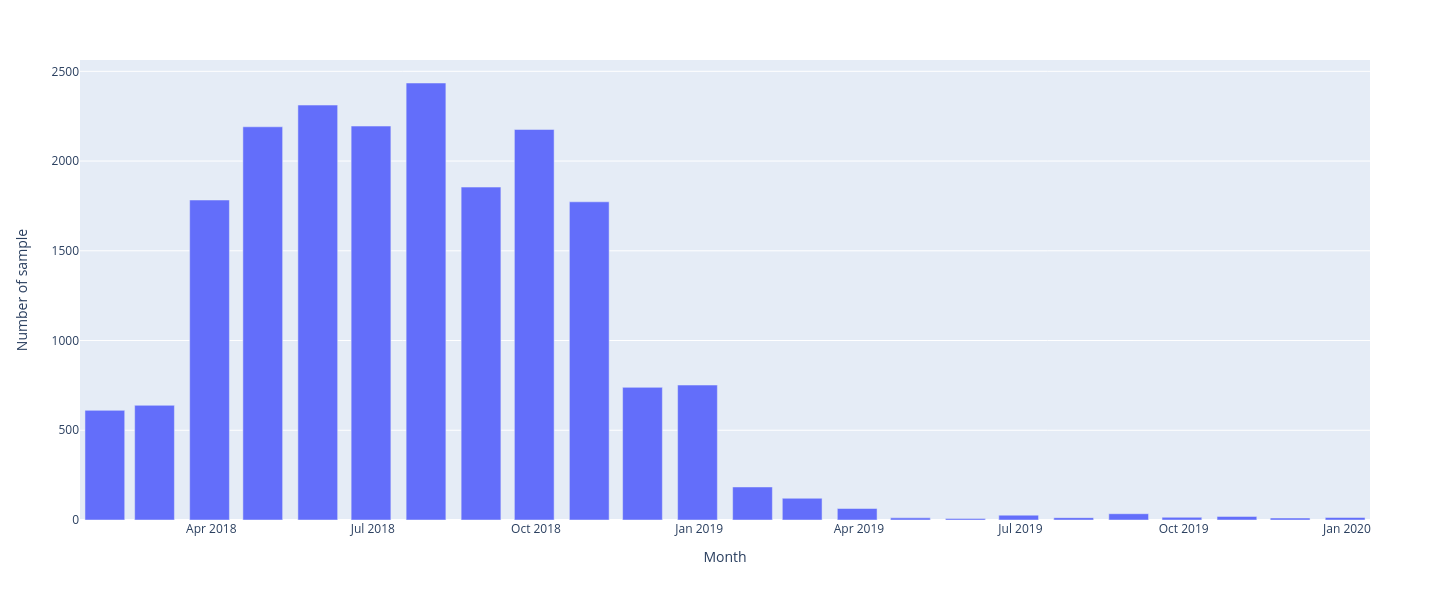
\includegraphics[scale=0.3]{sample_per_month}
    \centering
    \caption{Distribution des mesures par mois}
    \label{fig:figure2}
\end{figure}

Les mesures sont principalement concentrées entre Février 2018 et Avril 2019.
Aprés Avril 2019 la fréquence des mesures diminue.

\begin{figure}[H]
    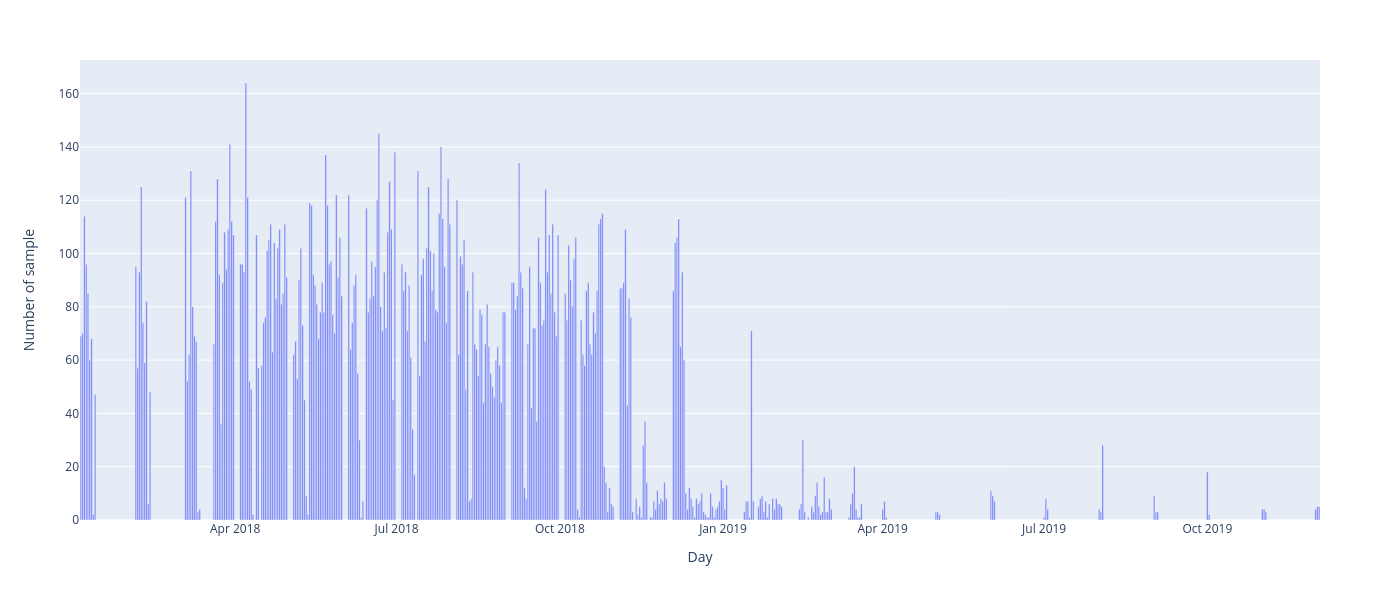
\includegraphics[scale=0.3]{sample_per_day}
    \centering
    \caption{Distribution des mesures par jour}
    \label{fig:figure3}
\end{figure}

Les mesures sont distribuées de manière irrégulières sur les jours de la période.

\begin{figure}[H]
    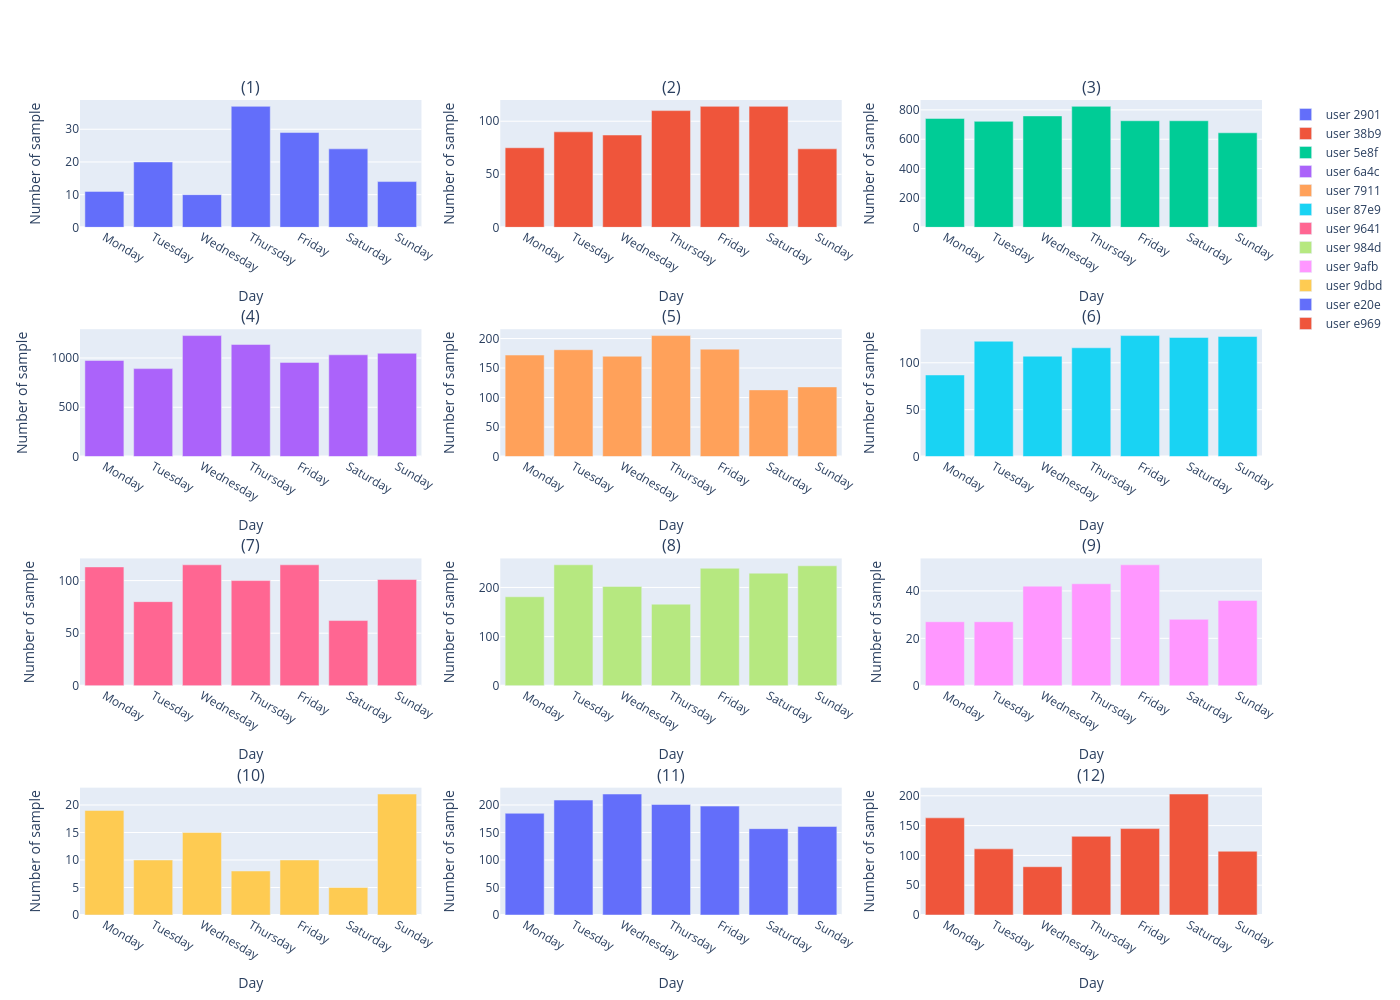
\includegraphics[scale=0.3]{sample_per_week_day}
    \centering
    \caption{Distribution des mesures par jour de la semaine par utilisateur}
    \label{fig:figure4}
\end{figure}

Pour certains utilisateurs les mesures sont distribuées de manière (presque) équiprobable (Figure 4.1, 4.2),
pour d'autres la répartition est irrégulière (Figure 4.8).

\begin{figure}[H]
    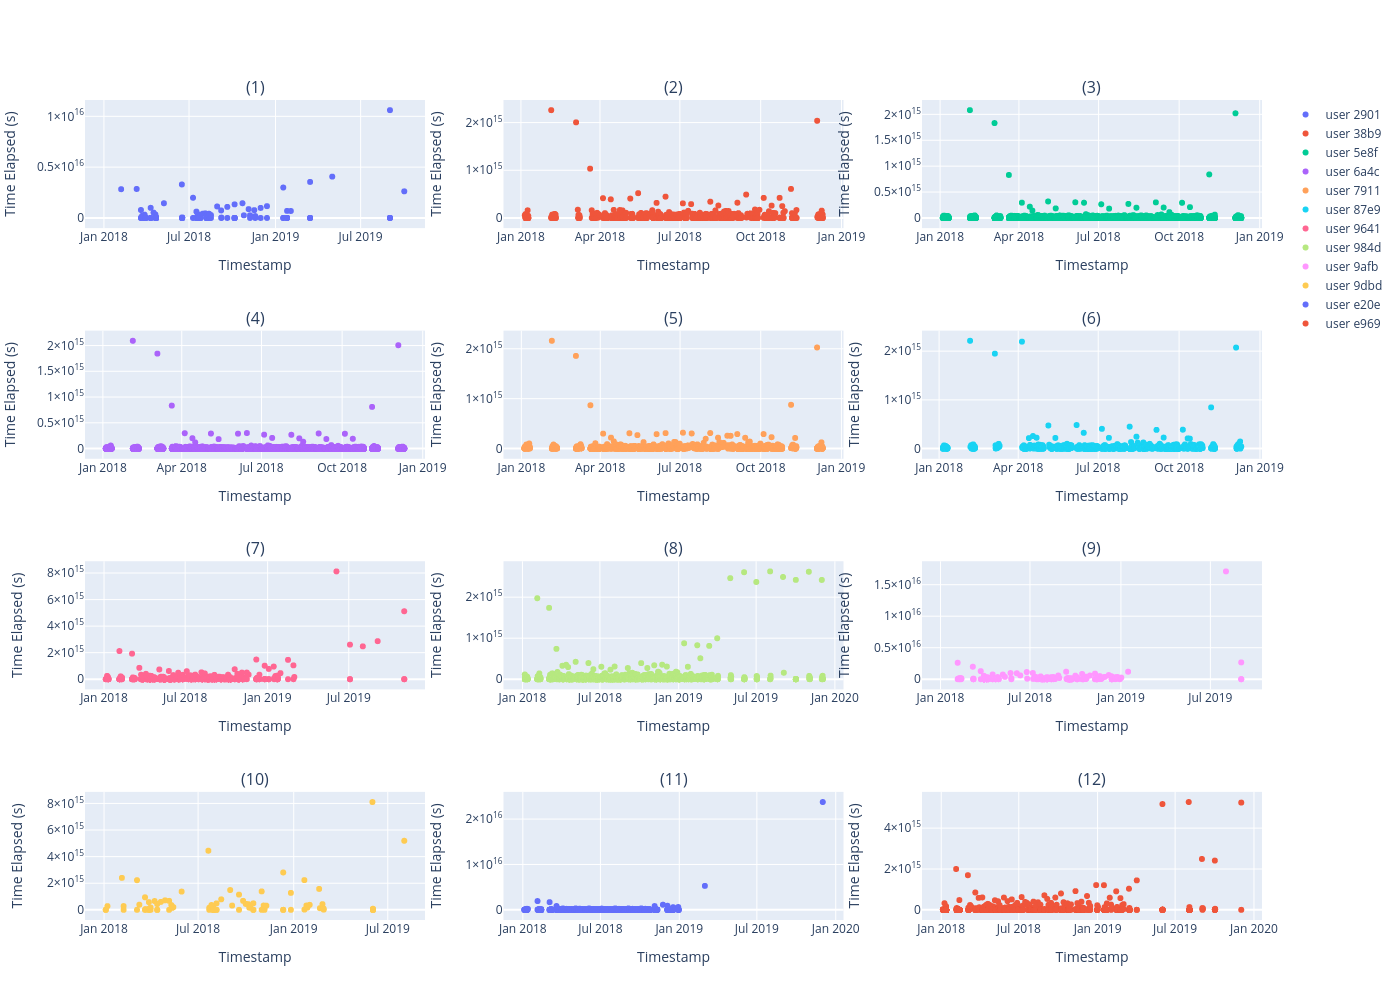
\includegraphics[scale=0.3]{time_elapse}
    \centering
    \caption{Distribution du temps écoulé entre deux mesures}
    \label{fig:figure5}
\end{figure}

Nous remarquons que pour chaque utilisateur il existe des points pour lesquels le temps écoulé est grand.
Cet écart peut être dû à des pertes de connections GPS ou des erreurs de localisation. Ces points engendrent du bruit
dans le jeu de données.

\vspace{5mm}
\subsection{Description Spatiale}

\begin{figure}[H]
    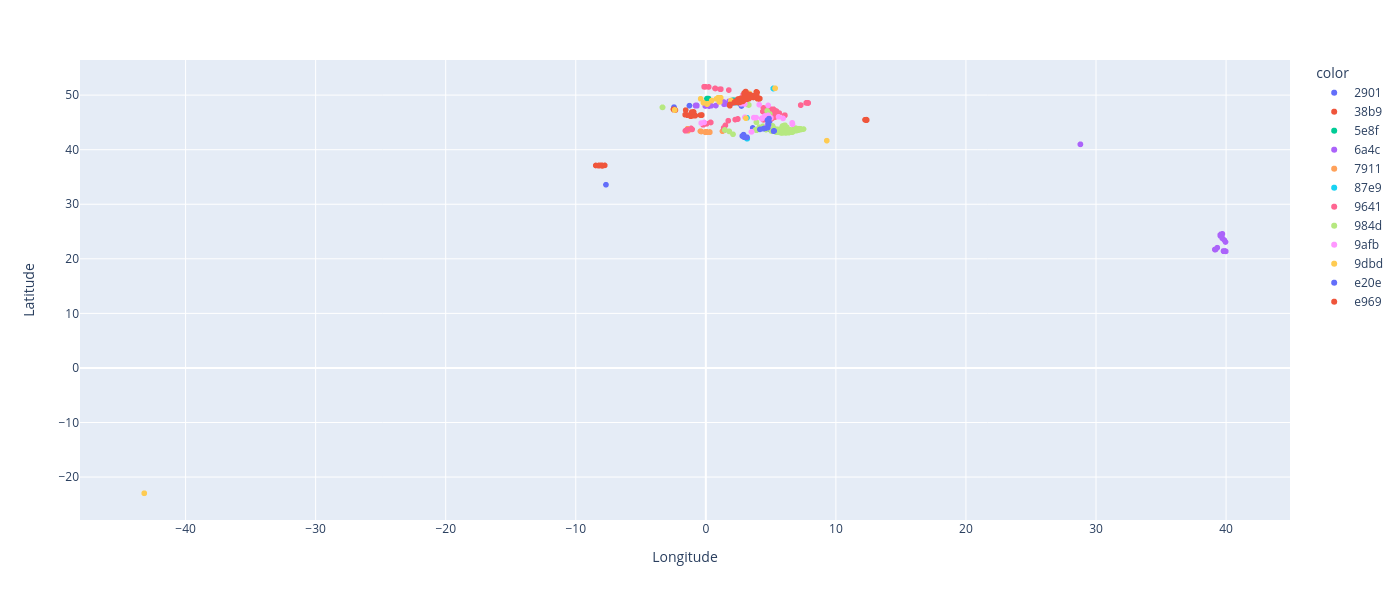
\includegraphics[scale=0.3]{gps_data}
    \centering
    \caption{Visualisation des données GPS}
    \label{fig:figure6}
\end{figure}

On remarque que le nuage de points est concentré autour d'une même zone géographique (pays par exemple).
Les utilisateurs proviennent tous d'une zone géographique proche.

\begin{figure}[H]
    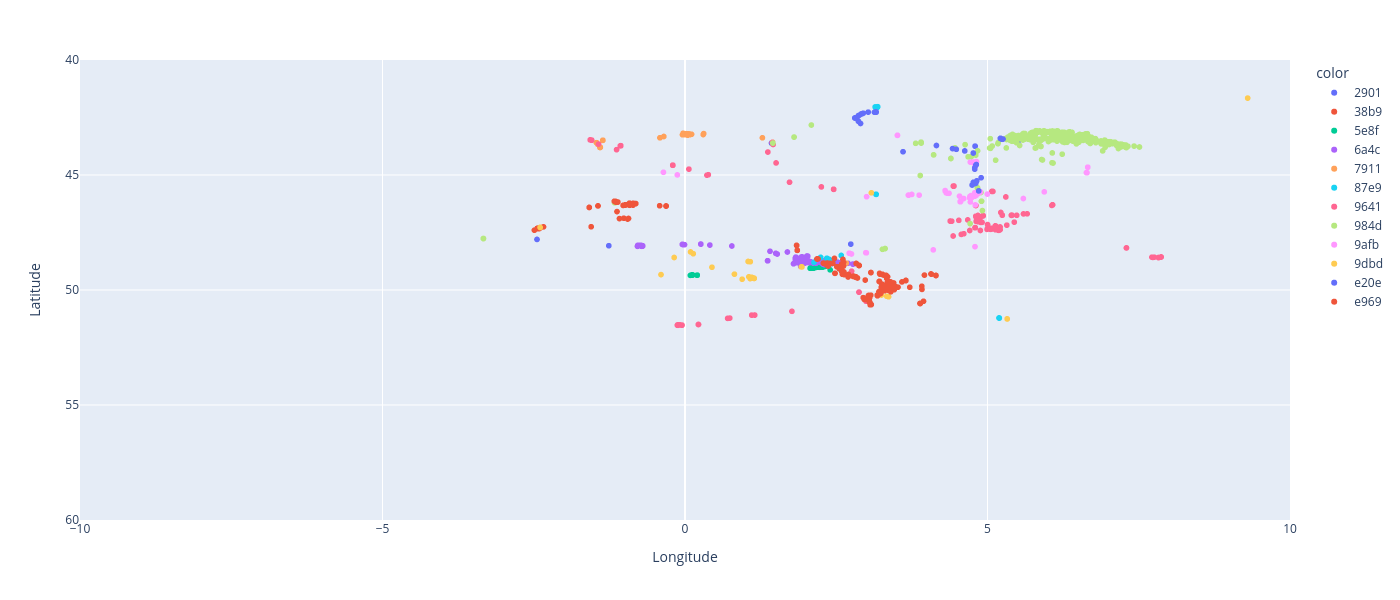
\includegraphics[scale=0.3]{gps_data_zoom}
    \centering
    \caption{Visualisation des données GPS (zoom)}
    \label{fig:figure7}
\end{figure}

On remarque que si pour certains utilisateurs les mesures GPS sont distantes,
pour d'autres les mesures sont confondues. Ces utilisateurs sont proches les uns des autres.
Il peut être difficile de séparer ces zones par clustering.

\begin{figure}[H]
    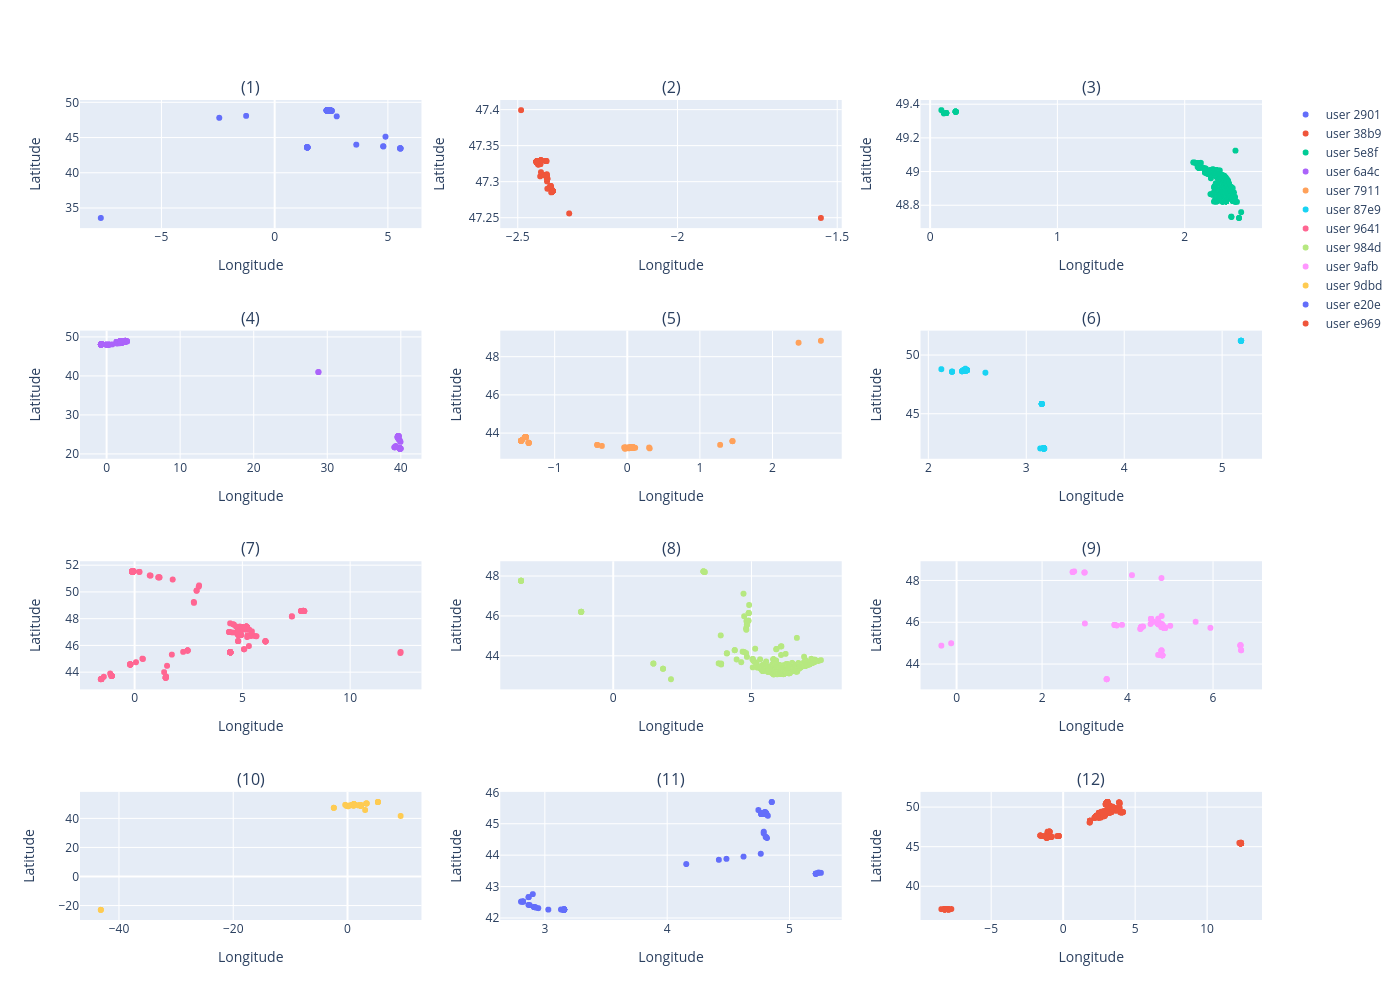
\includegraphics[scale=0.3]{gps_per_user}
    \centering
    \caption{Visualisation des données GPS par utilisateur}
    \label{fig:figure8}
\end{figure}

Pour chaque utilisateur, les nuages de points sont différents.
Pour certains utilisateurs (Figure 8.1, 8.5, 8.9) on distingue des zones denses,
tandis que pour d'autres (Figure 8.6, 8.11, 8.12) les points sont dispersés.


\begin{figure}[H]
    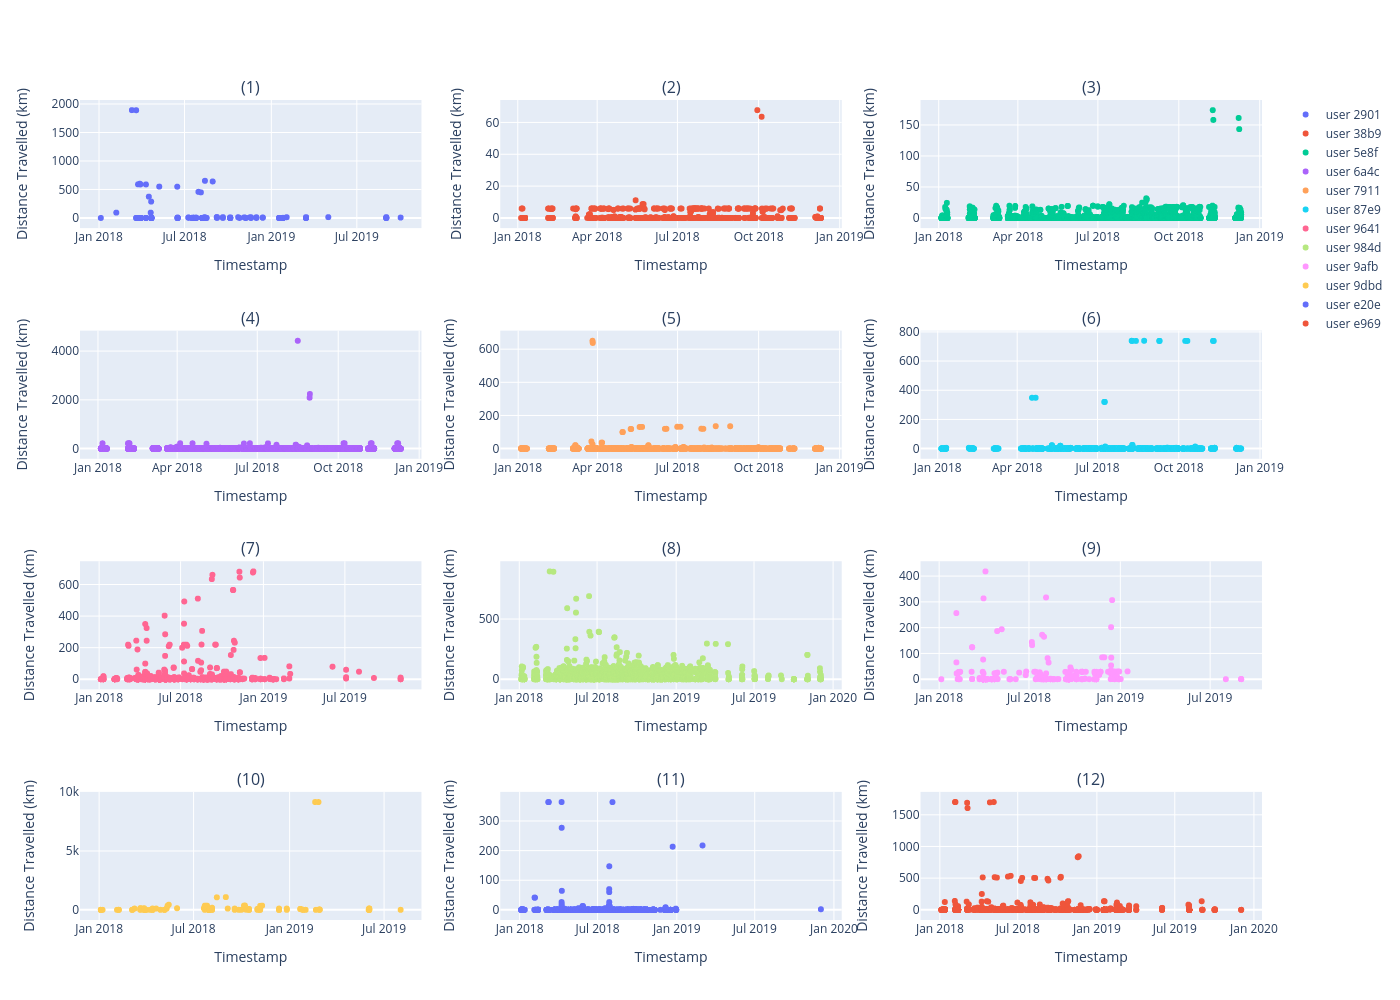
\includegraphics[scale=0.3]{distance_travelled}
    \centering
    \caption{Distribution de la distance (en km) entre deux mesures consécutives par utilisateur}
    \label{fig:figure9}
\end{figure}

De même que pour le temps, on remarque de grands écarts de distances entre les mesures.
Ces écarts peuvent êtres dû également à des pertes de connections ou des déplacements en transport.
Ces points bruitent également le jeu de données car nous sommes plus interessés ici par le temps passé dans un endroit
que le trajet pour y arriver.

\begin{figure}[H]
    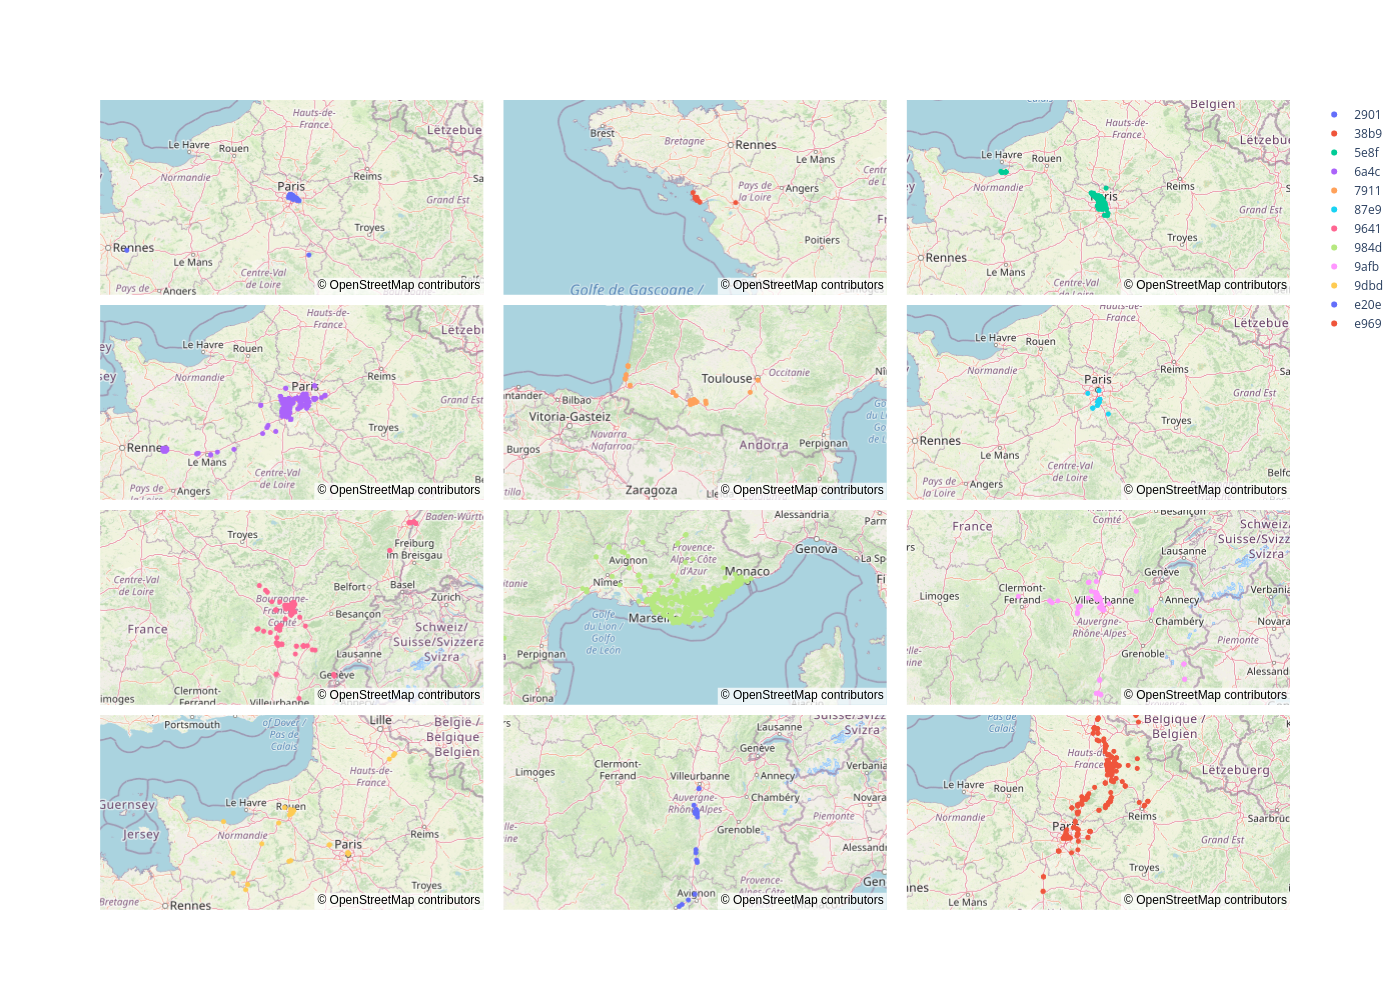
\includegraphics[scale=0.3]{map_view}
    \centering
    \caption{Vue cartographique des mesures GPS par utilisateur}
    \label{fig:figure10}
\end{figure}

Nous pouvons également visualiser la position et les déplacements des utilisateurs sur une carte.
Nous nous servirons de ces cartes pour vérifier visuellement les performances de notre approche.

\vspace{10mm}
\section{Modélisation}

\vspace{5mm}

\subsection{De quel type de problème d'apprentissage s'agit-il ?}

\vspace{5mm}
$\textbf{Réponse : }$

Dans ce projet nous devons prédire le lieu d'habitation des utilisateurs, comme nous ne disposons pas des lieux d'habitation des utilisateurs
il s'agit d'un problème d'apprentissage non-supervisé.
\vspace{5mm}

\subsection{Concevez un modèle simple permettant d'estimer le lieu d'habitation
    de l'utilisateur (latitude, longitude) en expliquant vos choix algorithmiques:
    hypothèses, feature engineering, choix de l'algorithme, hyperparamètres.}


\vspace{5mm}
$\textbf{Réponse : }$

Nous disposons dans ce jeu de données de mesure de la localisation des utilisateurs dans le temps.
Pour prédire le lieu d'habitation de l'utilisateur nous souhaitons regrouper les différents
emplacements où l'utilisateur a passé le plus de temps. Nous utiliserons donc des méthodes de
clustering afin de d'effectuer ce regroupement.
\vspace{5mm}

Pendant l'exploration de données nous avons remarqué que :
\begin{itemize}[label=\textbullet, font=\LARGE]
    \item La distribution des distances parcourues entre les points présente des valeurs extrêmes (grande distance entre les points),
          pouvant correspondre par exemple à des trajets en transport (avion, voiture)
    \item Certains enregistrements sur une période peuvent correspondre à des déplacements de l'utilisateur
    \item Les mesures ne sont pas régulières dans le temps
    \item Les localisations dépendent de la précision de l'appareil de mesure. Si un utilisateur reste au même endroit pendant un certain temps les données
          de latitude et longitude ne seront pas les mêmes (dispersion des valeurs)
\end{itemize}

Ces observations constituent un bruit dans le jeu de données. Afin d'améliorer la précision de notre prédiction
nous filtrerons ces valeurs.

\vspace{5mm}

Nous emploierons deux stratégies de filtrage, En notant $\textbf{L}_{i}^{j}$ la $\text{i}^{ème}$ mesure du $\text{j}^{ème}$ utilisateur :
\begin{itemize}[label=\textbullet, font=\LARGE]
    \item Filtrer les points ayant une distance parcourue supérieure à un certain seuil
          \begin{equation}
              \text{Si } \textbf{L}_{i-1}^{j} - \textbf{L}_{i}^{j} > \xi\text{, alors nous supprimons } \textbf{L}_{i}^{j}
          \end{equation}
          Dans le but de réduire le bruit généré par la mesure de l'appareil, le seuil ${\xi}$ devra être proche de l'incertitude de la mesure.
    \item Filtrer les points ayant une vitesse supérieure à la vitesse de marche moyenne.
          \begin{equation}
              \text{Si } \frac{\textbf{L}_{i-1}^{j} - \textbf{L}_{i}^{j}}{\Delta t_{i-1, i}} > \gamma\text{, alors nous supprimons } \textbf{L}_{i}^{j}
          \end{equation}
          Dans le but de réduire les points correspondant à des déplacements de l'utilisateur, ${\gamma}$ devra être proche de la vitesse de marche moyenne.

\end{itemize}

\vspace{5mm}

Pour déterminer l'incertitude liée aux mesures GPS, nous isolons un ensemble de mesures proches correspondant à l'emplacement d'un utilisateur (visualisé en Figure 10) grâce à un algorithme de clustering.
Nous calculons la distance moyenne entre les points de ce cluster pour obtenir notre estimation.

Pour la vitesse de marche moyenne, nous savons qu'elle est estimée entre 4 et 5 km/h. Nous choisirons 4.5km/h soit 1.25 m/s.


\vspace{5mm}

Même en supprimant l'ensemble de ces points, le jeu de données reste bruité. Afin de limiter l'impact du bruit
et puisque nous ne connaissons pas, a priori, le nombre de clusters, nous utiliserons
DBSCAN (Density-Based Spatial Clustering of Applications with Noise). DBSCAN présente l'avantage de clusteriser
par zone de densité et de créer un cluster 'Noise' pour détecter les valeurs aberrantes (outliers).

\vspace{5mm}

Trois hyperparamètres sont importants pour DBSCAN :
\begin{itemize}[label=\textbullet, font=\LARGE]
    \item ${\varepsilon}$, qui représente la distance maximum entre deux points pour qu'ils soient considérés comme voisins.
          Pour choisir nous utiliserons la méthode visuelle 'Elbow curve' puis nous validerons ces valeurs en nous aidant des maps (Figure 10).
          \begin{figure}[H]
              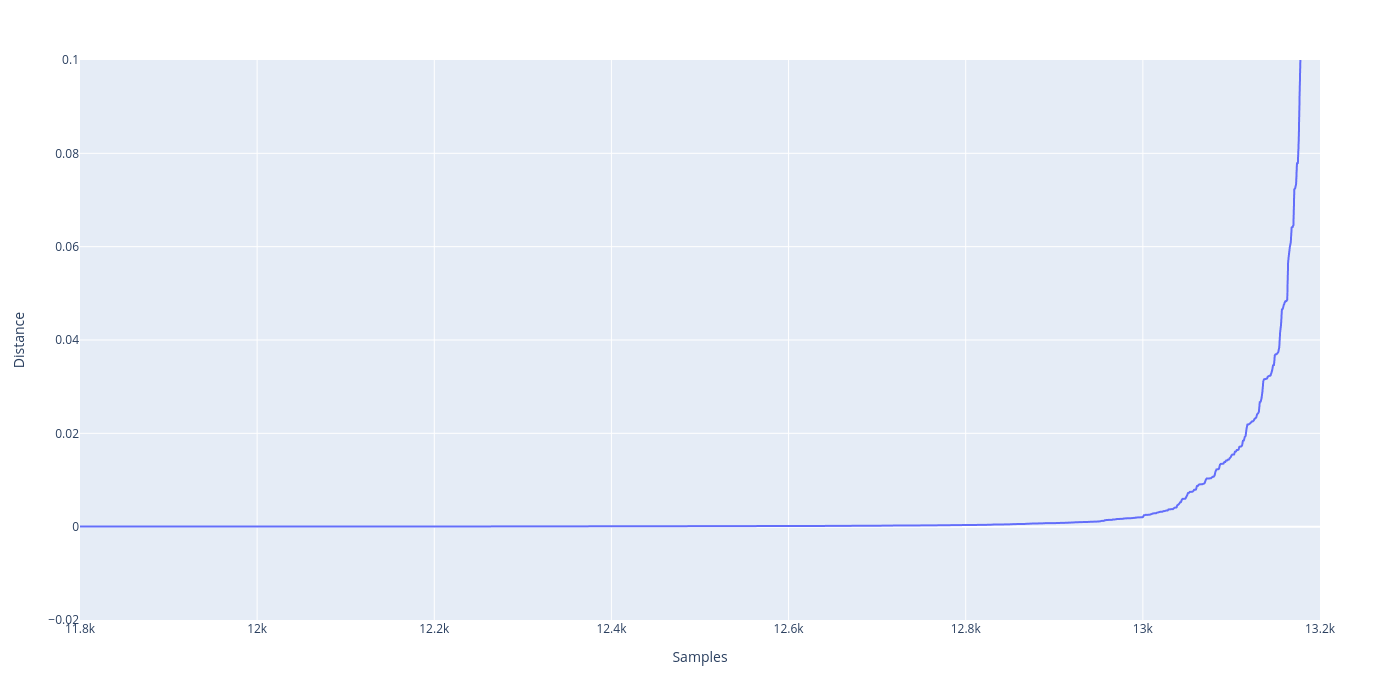
\includegraphics[scale=0.25]{elbow}
              \centering
              \caption{K-distance Elbow Curve}
              \label{fig:figure11}
          \end{figure}
          On trouve grâce à cette méthode ${\varepsilon = 0.040}$, cependant expériementalement cette valeur donne un mauvais résultat de clustering. On trouve empiriquement ${\varepsilon = 5.10^{-5}}$.
    \item min\_samples, qui représente le nombre de points dans un voisinage pour qu'un point soit considéré comme principal.
          Comme certains utilisateurs ont peu de points, min\_samples sera proche du nombre de mesures pour ces utilisateurs. Nous choisissons donc min\_samples = 3
    \item La mesure utilisée pour calculer la distance entre deux points. Nous utilisons la distance d'Haversine qui sert à calculer la distance entre deux coordonnées GPS.
\end{itemize}


\vspace{5mm}
Afin de prédire le lieu d'habitation des utilisateurs nous allons donc :
\begin{enumerate}[(1)]
    \item Nettoyer les données avec les stratégies évoquées précédement (Figure 12)
    \item Effectuer un clustering avec l'algorithme DBSCAN sur tous les utilisateurs (Figure 13, Figure 14)
    \item Récupérer pour chaque utilisateur le cluster le plus dense
    \item Estimer le centre du cluster (lieu d'habitation), en prenant le point du cluster qui a le plus de voisins proches
    \item Vérifier visuellement les performances de notre approche (Figure 15)
\end{enumerate}

\vspace{5mm}

\begin{figure}[H]
    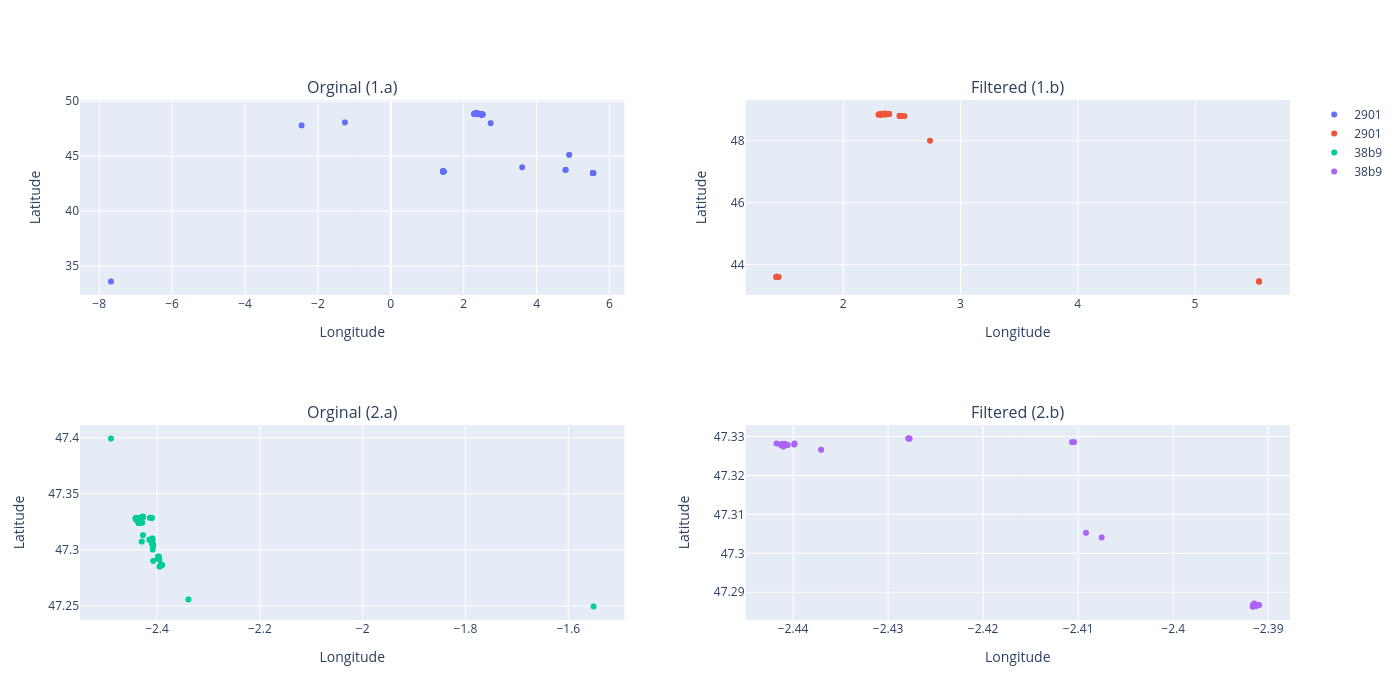
\includegraphics[scale=0.25]{viz_filtering}
    \centering
    \caption{Visualisation des données GPS avant (colonne de gauche) et aprés (colonne de droite) filtrage pour 4 utilisateurs}
    \label{fig:figure12}
\end{figure}

\begin{figure}[H]
    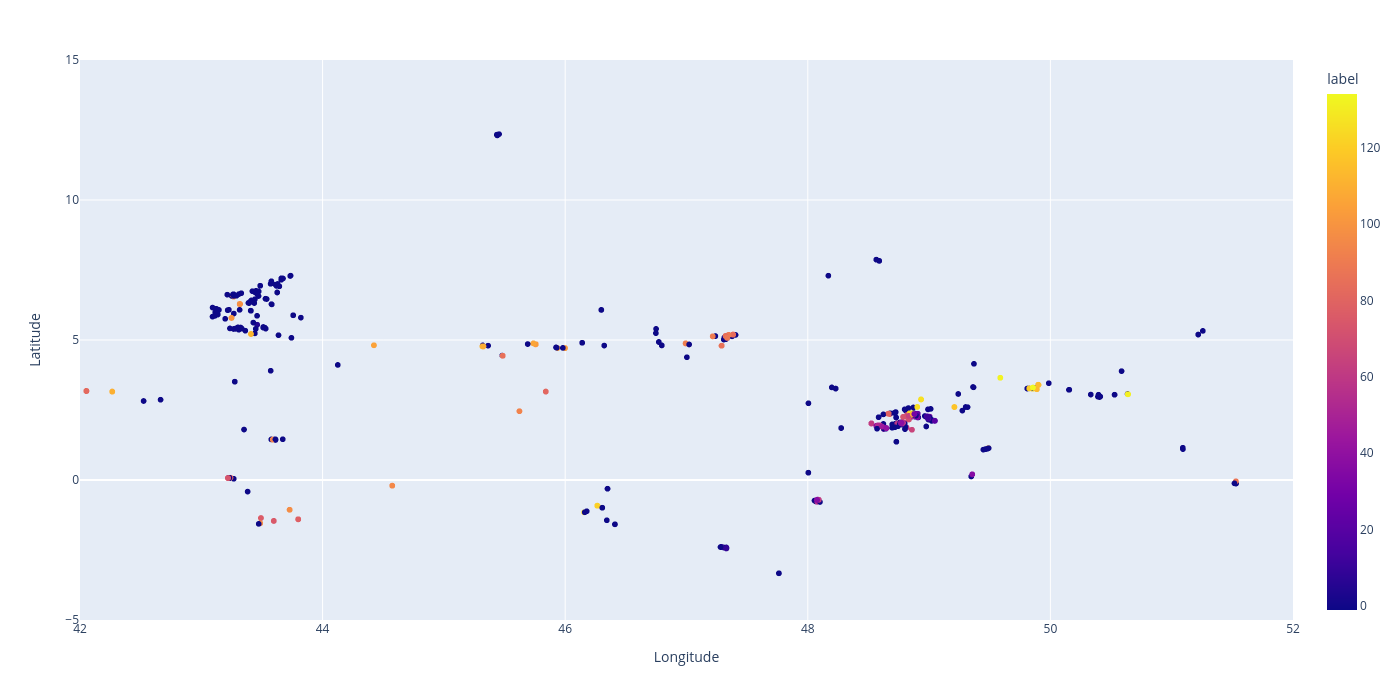
\includegraphics[scale=0.25]{DBSCAN_cluster}
    \centering
    \caption{Visualisation du clustering avec DBSCAN}
    \label{fig:figure13}
\end{figure}

\begin{figure}[H]
    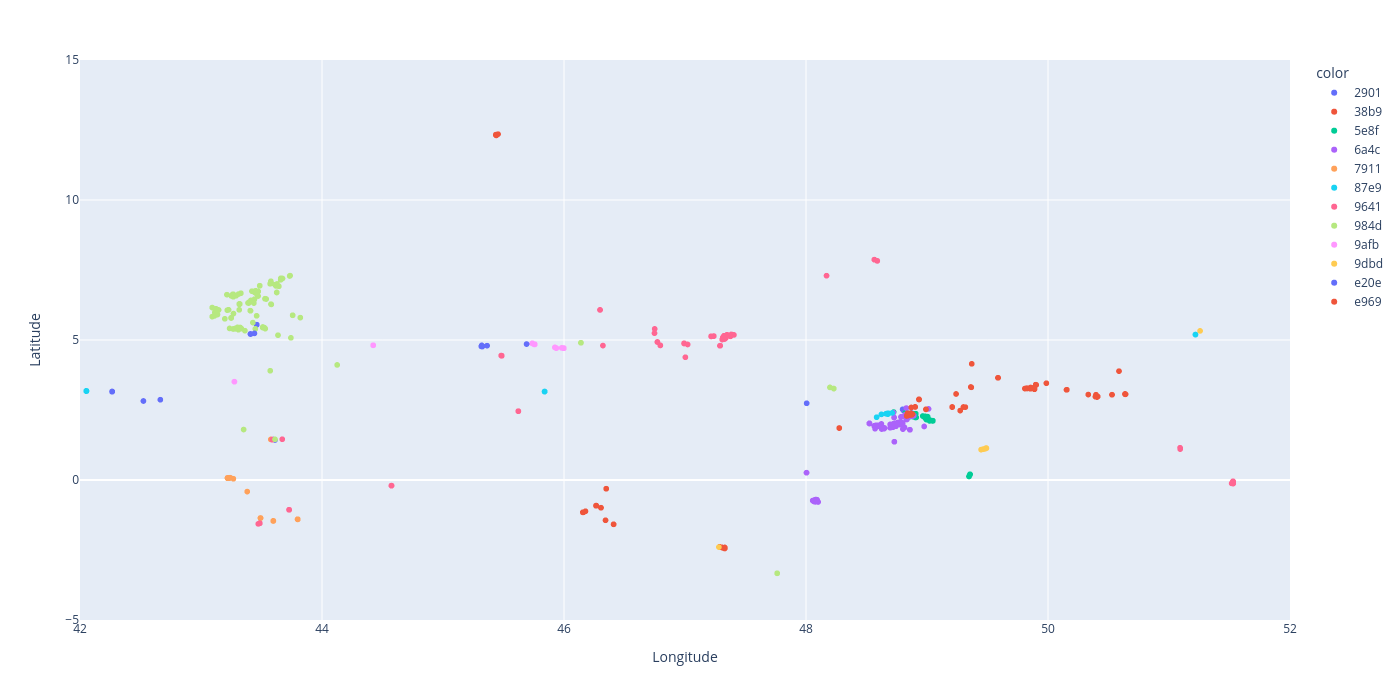
\includegraphics[scale=0.25]{user_cluster}
    \centering
    \caption{Visualisation du ground-truth clustering}
    \label{fig:figure14}
\end{figure}

\begin{figure}[H]
    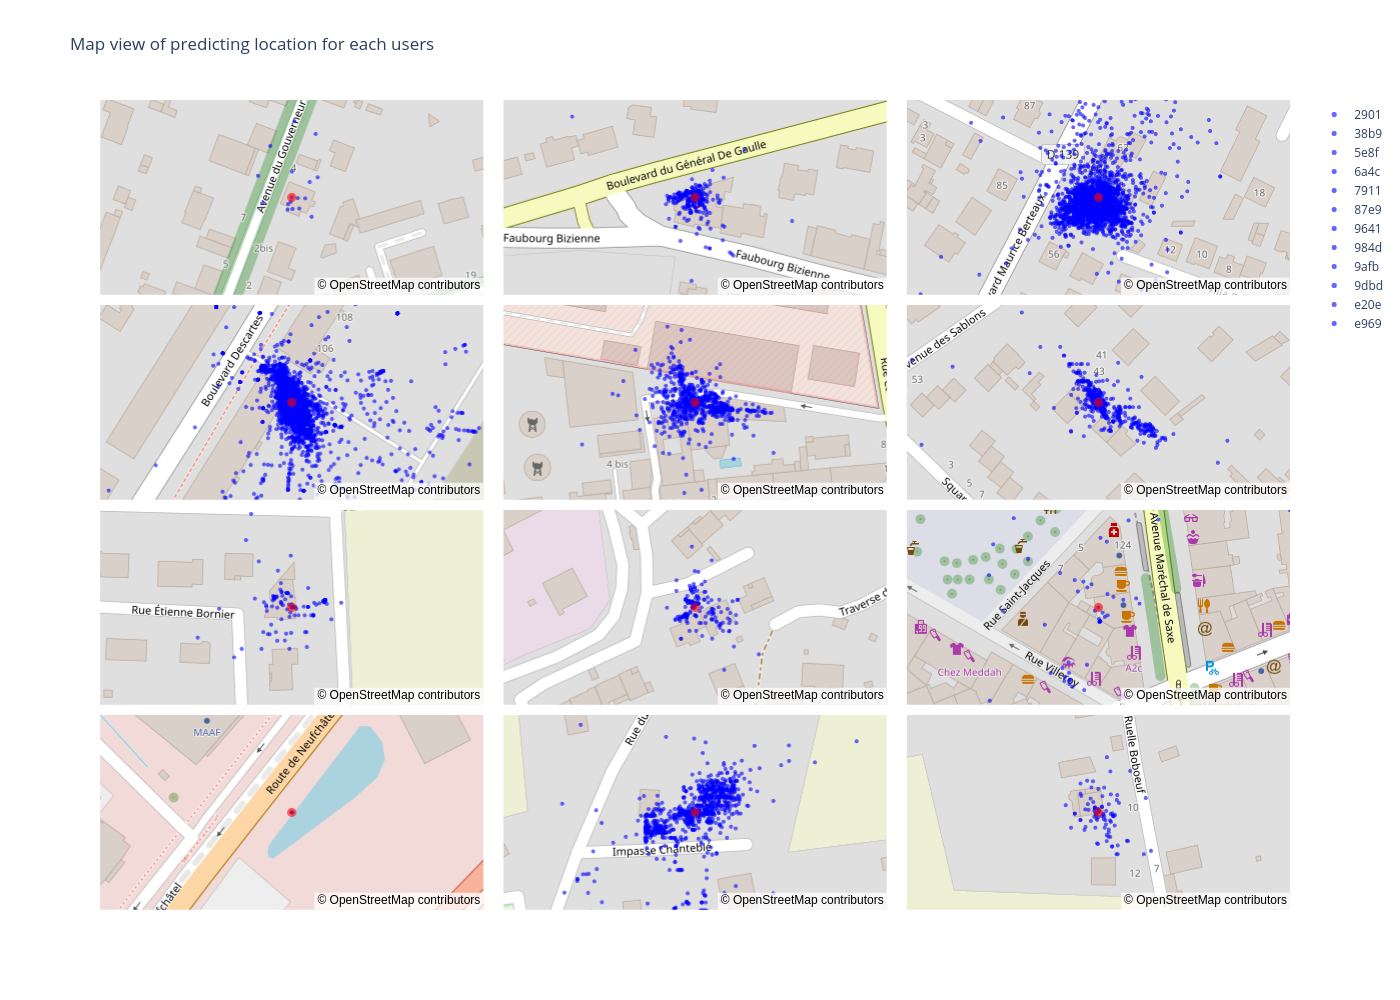
\includegraphics[scale=0.25]{map_prediction.png}
    \centering
    \caption{Vue cartographique des lieux d'habitation prédits pour chaque utilisateur}
    \label{fig:figure15}
\end{figure}


\subsection{Vous avez estimé le lieu d'habitation d'un utilisateur. Quelles informations complémentaires pourrait-on extraire de ce jeu de données ?}

\vspace{5mm}
$\textbf{Réponse : }$
\vspace{5mm}

Nous pourrions également extraire de ce jeu de données les sous-locations les plus fréquentées par un utilisateur (son lieu de travail, son magasin favori).
Aprés avoir identifié toutes les locations où l'utilisateur a l'habitude d'aller, nous pourrions nous servir des séries temporelles de trajectoire pour prédire
la localisation d'un utilisateur en fonction de l'heure et du jour de la semaine (GMM, Markov Models).


\vspace{5mm}

\subsection{Comment pourrait-on évaluer la performance du modèle (en faisant l'hypothèse que vous pouvez collecter des données supplémentaires) ?}

\vspace{5mm}
$\textbf{Réponse : }$
\vspace{5mm}

En faisant l'hypothèse que nous pouvons récolter le lieu d'habitation des utilisateurs et la précision/incertitude des appareils de localisation.
Nous pourrions labéliser les points du jeu de données qui seraient à une distance (incertitude de l'appareil) inférieure ou égale au lieu d'habitation.

Nous pourrions ainsi mesurer pour chaque utilisateur le nombre de points effectivement bien clusterisés et ainsi utiliser des mesures de performances de clustering (Homogeneity, Completeness ou  Mutual Information based scores).
Nous pourrions également mesurer l'écart entre la localisation GPS prédite et la localisation GPS réelle pour obtenir une mesure de la performance sur les coordonnées prédites (Mean Square Error)


\vspace{5mm}

\section{Bibliographie}

\begin{enumerate}[(1)]
    \item \textrm{\href{https://www.quadrant.io/resources/location-data}{Location Knowledge Base} }
    \item \textrm{\href{https://towardsdatascience.com/simple-gps-data-visualization-using-python-and-open-street-maps-50f992e9b676}{Simple GPS data visualization using Python and Open Street Maps} }
    \item \textrm{\href{http://danielashbrook.com/pubs/2003 Ashbrook-Using GPS to Learn Significant Locations.pdf}{Using GPS to Learn Significant Locations and Predict Movement Across
                  Multiple Users} }
    \item \textrm{\href{https://www.ncbi.nlm.nih.gov/pmc/articles/PMC6242315/}{A geographical location prediction method based on continuous time series Markov model} }
    \item \textrm{\href{https://hrngok.github.io/posts/gps-data-analysis/}{GPS Data Analysis}}


          \vspace{5mm}
\end{enumerate}


\end{document}

